\chapter{Einfügen in einen Suchbaum II}

\section*{Lösung}

Der gesuchte Baum lässt sich mit den in Abschnitt~\ref{ch:binarytree} aufgeführten Kriterien durch sukzessives Einfügen der Schlüssel konstruieren (s. Abbildung~\ref{fig:tree}):


\begin{figure}[h]

    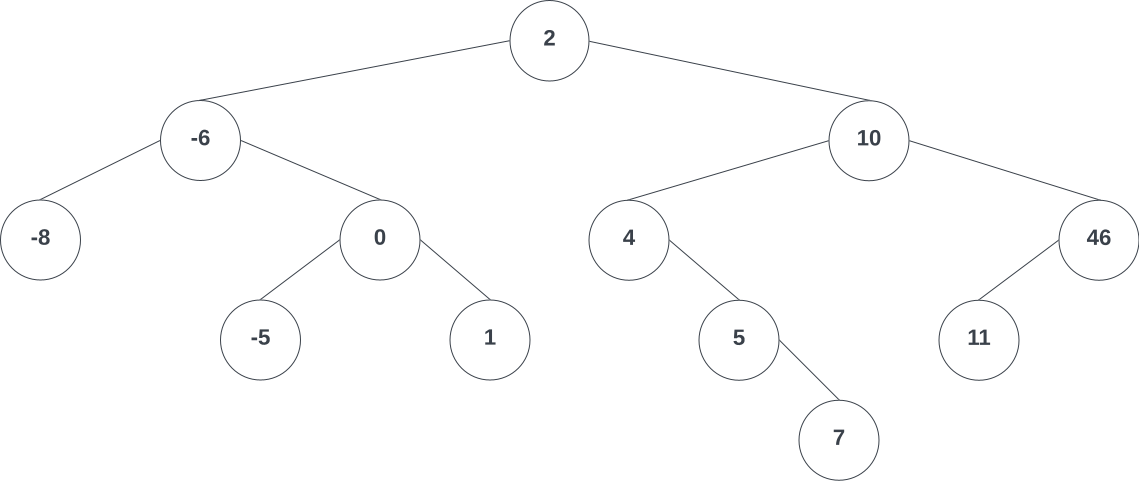
\includegraphics[
        width=16cm,
        keepaspectratio,
    ]{chapters/7. Einfügen in einen Suchbaum II/img/tree}
    \caption{Der Suchbaum nach Einfügen der Folge $2, 10, -6, 4, 46, 0, 5, -5, 7, -8, 11, 1$.}

    \label{fig:tree}
\end{figure}
